\documentclass[border=10pt]{standalone}
\usepackage{pgfplots}
\pgfplotsset{compat=1.18}
\begin{document}
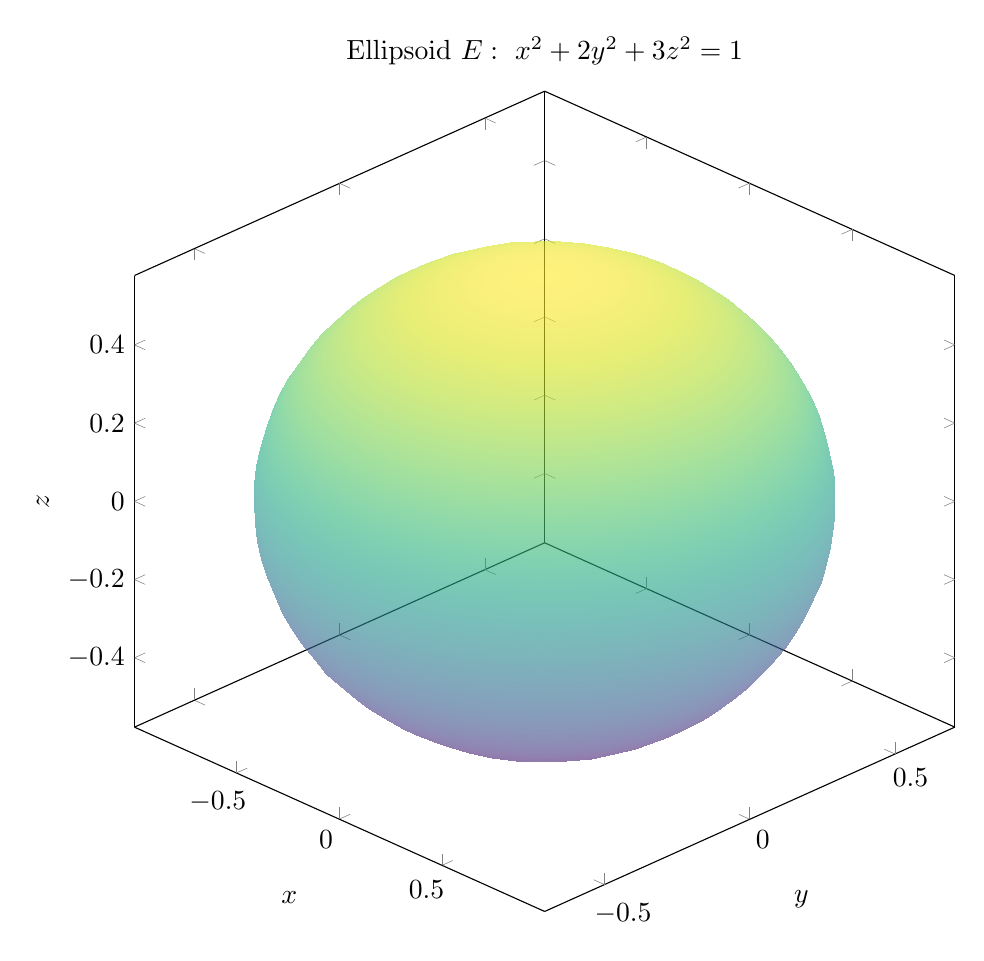
\begin{tikzpicture}
\begin{axis}[
    title={Ellipsoid $E:\ x^2+2y^2+3z^2=1$},
    xlabel={$x$}, ylabel={$y$}, zlabel={$z$},
    width=12cm, height=12cm,
    view={45}{30},
    colormap/viridis,
    enlargelimits=false,
]
% Parametrize the ellipsoid
\addplot3[
    surf, shader=interp,
    domain=0:180, domain y=0:360,
    samples=40, samples y=40,
    z buffer=sort,
    opacity=0.6,
] (
    {sin(x)*cos(y)},
    {sin(x)*sin(y)/sqrt(2)},
    {cos(x)/sqrt(3)}
);
\end{axis}
\end{tikzpicture}
\end{document}